\documentclass[notitlepage]{report}
\usepackage{graphicx, multicol, float}
\usepackage[margin=1in]{geometry}
\usepackage{titling}
\usepackage[dvipsnames]{xcolor}
\usepackage{amsmath}
\usepackage{amssymb}
\usepackage[normalem]{ulem}
\usepackage{listings}
\usepackage{xcolor}
\useunder{\uline}{\ul}{}
\begin{document}

\pretitle{\begin{center}\Huge\bfseries\vspace*{5em}}
\posttitle{\par\end{center}\vskip 0.5em}
\postdate{\end{center}\vspace*{7em}}

\title{Steganography in digital media}

\author{
	Pricope Stefan-Cristian\\
	\texttt{psir2384@scs.ubbcluj.ro}
  	\and
  	Dr. Suciu Mihai\\
  	\texttt{mihai-suciu@cs.ubbcluj.ro}
}
\date{\vspace{-6ex}}
\maketitle
\thispagestyle{empty}

%Abstract - small description of the paper
\begin{abstract}
Steganography is the science of concealing a piece of information within another piece of information without affecting the latter in a noticeable way and therefore alerting any intruders of the existence of the former. 
This paper presents both existing and new ways of embedding computer files and data into different digital multimedia formats as covert as possible while still allowing the encoded information to be retrieved at a later time without any significant losses.
\end{abstract}


%Aici vine cuprinsu
\tableofcontents{}

%Aici incep capitolele

\chapter{Introduction to computer steganography}
%\section{Introduction to computer steganography}

\setlength\columnsep{20pt}
\begin{multicols*}{2}
The practice of hiding and securing information and messages between different parties has played a major part alongside human history, especially during times of war when it was vital that the enemy didn't intercept the strategies and even if they did, they would have no idea what to do with them and would have to dedicate a lot of time, money and personnel to decode the communications. Two of the most famous manifestations of this practice are cryptography and steganography\cite{steganography-history}.

Trying to differentiate between cryptography and steganography is not difficult, the only thing they have in common is their end goal - making sure that a piece of information sent from one place to another is secured and that only the right recipient will be able to read and understand the received information. The difference lies in the methods they use and the time it takes to reach that goal.

Cryptography focuses on altering the information itself, encrypting it using a key only known by the receiver and sender\footnote{This is only true in symmetric cryptography and is a gross oversimplification of cryptography as a science, but it is just meant to get a point across and help differentiate between the 2.}, making it harder for any possible meddlers to  alter the meaning of the message or even just understand it. Steganography is more concerned on hiding the fact that there even is any information being transmitted usually by embedding it in something else (hereby referred to as a cover), thus if any interlopers were to actually look at the cover, they wouldn't even be aware of the fact that it contained secrets.

In other words, both methods are meant to be used over an open and unsafe environment, and while cryptography tries to hide the contents of the message but not the fact that there is a message being sent, steganography tries to hide the communication altogether. The main advantage of these 2 methods is that they are not exclusive, they can be used together for maximum safety of the information.\footnote{The speed of encoding/decoding the information is greatly decreased when these 2 are combined which is the reason that nobody merges them, preferring to juse use encryption to keep the information safe.}

%Given the evolution of the Internet and computers in general in the last 5 decades, there was a need for keeping the communications secure over all the networks, especially in the last 2 decades when computers became common household items. Thus, cryptography really got to shine and thousands of algorithms for encrypting the information were conceived and the very few remarkable ones are still being used\footnote{The reason cryptography is in the spotlight is because it is much faster, mathematically proven, and it hides all the data without leaving anything in plain sight(like steganography does with the cover)}.  But that doesn't mean steganography was left behind, quite on the contrary, researchers developed plenty of new algorithms for hiding information using digital files as cover.

With the evolution of the Internet and the increasing usage of personal computers in day to day activities we needed to secure the data sent over the network between the users. The efforts were lead by cryptographers who developed thousands of algorithms for encrypting the information and the very few remarkable ones are still being used\footnote{The reason cryptography is in the spotlight is because it is much faster, mathematically proven, and it hides all the data without leaving anything in plain sight(like steganography does with the cover).}.  But that doesn't mean steganography was left behind, researchers developed plenty of new algorithms for hiding information using digital files as a cover and the Internet as the transmission environment.

In theory all types of digital files can be used as cover  - shared libraries and executables can be edited to include the hidden data and then be recompiled/rebuilt, text files and documents could be modified to enclose the information in secret places/paragraphs, and multimedia such as images, music and video files can be changed to carry the digital data into their metadata, pixels, audio frequencies, motion vectors and much more. This paper will go into details about some of the most popular formats used for multimedia files and showcase their internal structure and document techniques used in steganography.
\end{multicols*}





\chapter{Steganography methods}


\section{Least Significant Bit(LSB) Insertion} \label{lsb_insertion_chapter}
\begin{multicols*}{2}
\subsection{Sequential}
\setlength\columnsep{20pt}

Least Significant Bit or LSB is by far the most used method when talking about any type of steganography. Given that the smallest unit a computer can understand and process is usually a byte, altering only the least significant bit will not change the transmitted information in a noticeable way to any external parties. It is much easier to showcase what a byte contains and what the LSB change implies and how it works. A byte contains 8 bits, so this means that the values a byte can take range anywhere from 0 to 255 (inclusive)\footnote{This is the case for unsigned bytes, but given that we are talking about a method that only deals with the least significant bit, we can safely ignore the most significant bit, also known as the sign bit.}. Let's assume that we have an array of 4 random values in consecutive memory : 217, 127, 100, 62 (all values are in decimal), each stored on exactly one byte, and that we want to hide our grade in Numerical Analysis from our parents (in this case a 3) using a LSB substitution.
\begin{figure}[H]
    \centering
    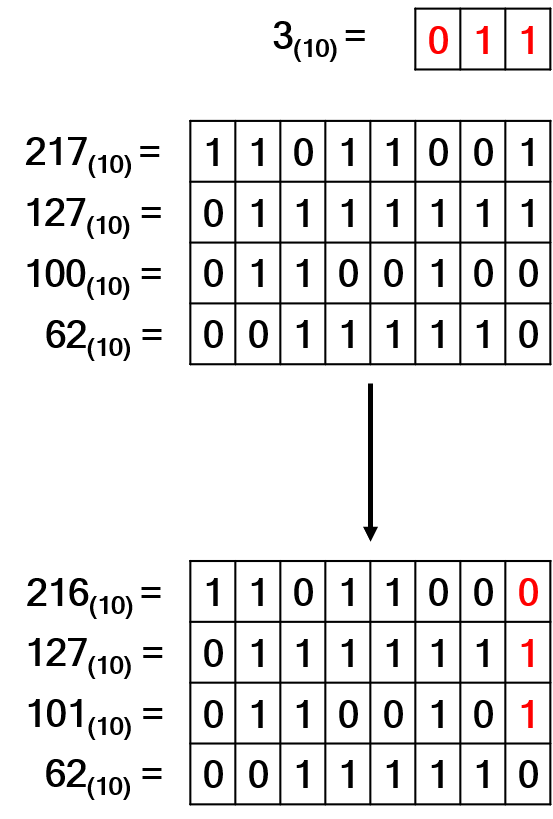
\includegraphics[width=2.8cm,keepaspectratio]{pics/how_lsb_works}
    \caption{How the sequential Least Significant Bit change works}
    \label{LSB}
\end{figure}

As we can see from Figure \ref{LSB}, we have succesfully altered the least significant bit of the first 3 bytes of the stream in order to hide our grade : 217 became 216 when we changed the last bit from 1 to 0, 127 was unchanged because it already had the last bit set, and the third byte became 101 after toggling the final bit. Furthermore, the rest of the stream (the fourth byte, 62) was not affected because we already hid the entirety of our secret message. While this is great because we only hide exactly as much as we need and not a byte more, we have a high risk of corrupting the hidden message in case our cover image gets compressed or loses even a single byte when sent over a network. Basically, we are trading data redundancy in order to get simplicity and efficiency.

Sequential LSB insertion is the simplest and most common way of embedding any kind of information into a byte stream that is then shared. It has been thoroughly discussed by a great deal of researchers and has been the subject of many papers where it was analyzed and benchmarked\cite{seeing-the-unseen}\cite{hide-and-seek} . Being the most popular technique also means that any flaws the method has are widely documented and showcased. Steganalysis\footnote{Steganalysis is the study of steganographic methods, including but not limited to : differences in file sizes or in color histograms, secret message redundancy, embedding capacity and performance etc.} performed on outputs created using this algorithm has shown that it is unreliable to stay undetected if an outside party intercepted the message containing the cover file\cite{attack-on-steganography}. Furthermore, doing a simple reverse engineering on the algorithm reveals even more issues with this naive encoding : if a single bit that is part of the secret message was flipped from the cover file byte stream, the message would become corrupted and the original secret would be lost forever. This means that sequential LSB insertion is not resistant at all to any form of lossy compression where some of the original data may be lost in order to reduce the used disk space because it would lose most, if not all, of the embedded file information. 

Furthermore, it is extremely easy to compute the carrier storage, i.e. how many bytes we are able to hide into the cover file or in other words, the maximum size of the secret message that we can succesfully embed without losing anything while still keeping a covert profile. Assuming $CDS$ or Cover Data Size (how many bytes are actually used to store the pixel information, no metadata information or chunk headers or anything like that), then the $MMS$ or Maximum Message Size would be equal to

\[ MMS = [CDS \ / \ 8] \ bytes \]

or the integer part of CDS divided by 8. This should come as no surprise since sequential LSB is altering $1/8$ (an eighth) of each byte when embedding a bit of the secret information so the maximum capacity makes sense to also be $1/8$.


\subsection{Scrambling} \label{scrambling_chapter}
As documented earlier, sequential LSB insertion algorithm has a decent number of flaws so it was needed to develop some new techniques that are not relying as much on the cover file not losing a few bytes or undergoing a compression algorithm. In other words, it needed to introduce a few redundancies to ensure that the secret message wouldn't be lost as easily and that the message was not written in a sequential and direct order. They achieved this by not just changing the least significant bit in a sequential order, but by writing in an apparently random order (in simpler terms, scrambled) that could be reproduced by having the right key or by using the same algorithm in order to retrieve the embedded information. In this subsection we will discuss a few of the most common scrambling techniques and introduce a new one as well.

The most popular methods used for scrambling secret messages into various covers usually choose to simply ignore the entire data stream and only focus on a specific subsection and choose that as the carrier environment. After a smaller subsection is chosen (it can still be the entire actual data part of the cover, it's not an actual rule), we will have to generate the order in which we will write the message information. As mentioned before, this is derived using a key known only to the sender and the receiver that can be shared between the 2 parties using another transmission environment, preferably one that is encrypted and safe. The main logic is to use that passkey as a seed in a valid pseudo random engine when generating the order so that there are no collisions and that only the right key will produce the right order. 

There is also an option for when there is no safe method of transmitting a key and that is to scramble the secret message within a certain order that is not sequential. But as long as the receiver and transmitter have no way of communicating the algorithm used in embedding the message (can also assume this because they have no way of sharing the key), this option is useless but is still interesting to look into because they are a variation of the other mentioned option. Having no key to generate the order makes this option easier to showcase(since we don't have to also simulate a pseudo-random engine and a seed). Let's assume we have a byte stream of random data\footnote{Now the actual data meaning can be safely ignored because we only work on the LSB and we have seen in the previous chapter it does not alter the data in a significant way such that an intruder might notice something is wrong.} and we want to again hide a grade from our parents, in this case a 6 (or 110 in binary). Instead of hiding the grade sequentially, the bits will be hidden into the last bit of every third byte and it will end up looking something like this :

\begin{figure}[H]
    \centering
    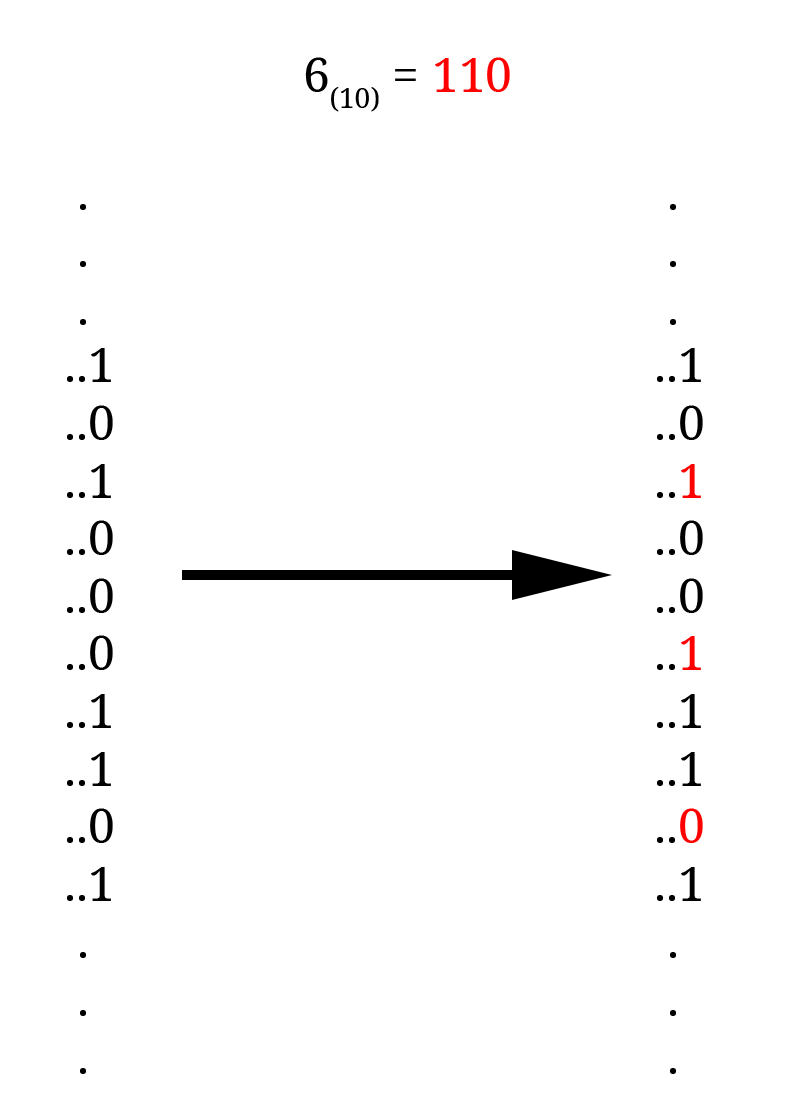
\includegraphics[width=5cm,keepaspectratio]{pics/scrambling_example}
    \caption{An example of scrambling LSB insertion}
    \label{Scrambled LSB}
\end{figure}

The key difference from sequential LSB insertion is that as long as the sender and receiver are aware of the used algorithm, any external parties will not be aware of the secret embedded message. Furthermore, this method has proven very useful because there are infinite ways of scrambling a message into the cover file without alerting any possible intruders and it ends up being an extremely hard guessing game for the attackers in their goal to extract the information.

The carrier capacity appears initially to be the same, but it is very important to remember that the scrambling algorithm used will usually work on a subset of the cover data bytes, not the entirety of it (just like in figure 2.2 we used only each third byte to store the information). Using the same notations as in the previous chapter we get that 

\[ MMS \leq [CDS \ / \ 8] \ bytes \]

so in most cases, the scrambled MMS will be smaller than the sequential MMS. However it is very important to note that this decrease in size comes with a great increase in data security and message safety.

This paper also introduces a new type of scrambling algorithm created by the authors that only works on lossless image formats that do not use any kind of interlacing when rendering the picture. It relies on scrambling the secret message into the image sub-blocks in a specific order that can only be deduced by having the right passkey. More information on this method is presented in chapter 3.2.1 after the introduction of image basics.


\section{Metadata encoding}
The word metadata was formed from combining the word "data" with the prefix "meta-" and is used to describe a special type of data that has information about other types of data\cite{metadata-origin}. In simpler terms, it means "data about data" and it keeps the same meaning in the digital world. It is much easier to visualize and understand the concept of metadata using a simple example : let's take a picture stored on a computer.

\begin{figure}[H]
    \centering
    
\includegraphics[width=2.3cm,keepaspectratio]{pics/goose_file}
    \caption{A simple image file}
    \label{Goose Image File}
\end{figure}

As noted in the introductory chapter, every file can be seen as a byte stream. However it is very important to keep in mind that those bytes don't represent only the image data, the pixels seen on the screen, they are much more. They also contain information about the camera used to take the photo, the location where it was taken, when the file was created, when it was modified, etc. All of the aforementioned information forms the metadata. It varies from file format to file format where they store this information in the byte stream, how many bytes are allocated for each piece of information or if it even has any effects on the actual file data. Most of the time metadata fields are only parsed by the renderer software and are mostly hidden to the user, but there are a few ways of viewing the information: 
\begin{itemize}
  \item using a hex editor to view the raw bytes of the file and then mapping those bytes to the publicly available file format specifier - an international approved paper which specifies the meaning of the bytes in the file binary stream
  \item using the operating system to view more properties about the file, not just the actual data interpreted and displayed to the end user
  \item using a third party tool which already knows the mapping and meaning of each sequence of bytes in the file binary stream and can succesfully parse the metadata
\end{itemize}

\begin{figure}[H]
    \centering
    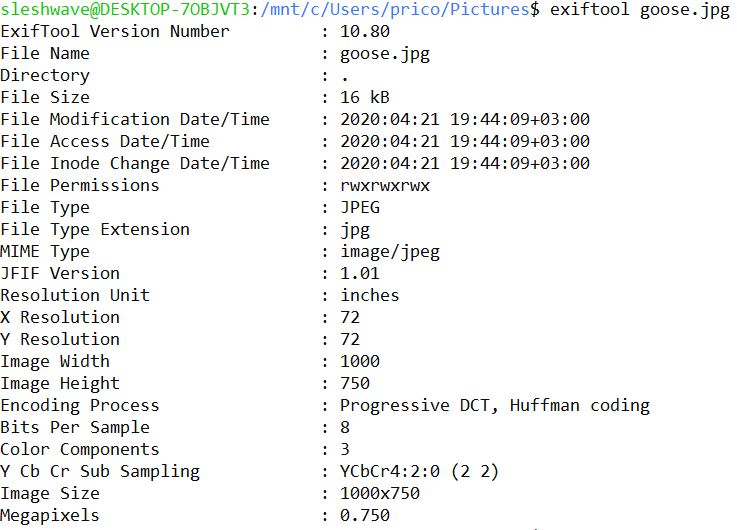
\includegraphics[width=8cm,keepaspectratio]{pics/exiftool_file_metadata}
    \caption{Example of using a tool to read file metadata}
    \label{Goose Image File Metadata using Exiftool}
\end{figure}

The focus of this sub-chapter will be on the metadata fields that don't necessarily have any important effect on the data representation and theoretically could be altered, such as any comments from the author or any contact information. In the case of an image, changing important metadata fields such as the width or height of the picture are not very covert methods of embedding any information at all, proving that not all fields are equally important. We are left with the more \textit{useless} metadata fields, but the good news is that most file formats allow these fields to have a variable size which is perfect for any steganographic purposes because it removes the size constraint of the secret message. While in theory this allows for $\infty$ MMS, there are a few limitations in place that significantly reduce that number: 
\begin{itemize}
  \item computers have a limited amount of storage space, in most modern day computers that would be about one terabyte. This means that the MMS will certainly be smaller than that.
  \item most file formats that allow metadata fields to be embedded in the byte stream of the file by an external party also have a sequence of bytes that indicates how long that metadata field is (how many bytes it contains). In most cases that sequence is 4 bytes long so this usually results in a MMS of $2^{4*8} = 2^{32} \approx 4.29\ gigabytes$.
  \item in the pursuit of keeping the existence of a secret inside the cover file as covert as possible, the MMS is again limited by the CDS. This happens because the size of the cover file is almost always displayed to any parties without any interactions and it needs to not raise any suspicions or attract unwanted attention to the actual contents of the file. To give an example, it would be very weird to see a simple image in FULL HD resolution have a size of two gigabytes and will almost certainly alert any intruders. It is extremely hard to say an exact MMS based on this limitation because it depends on the original cover file size and it should be relative to that number. It is recommended that $MMS \leq  50\% * CDS$.
\end{itemize}

In the end it is important to note that metadata secret encoding is the most trivial method of embedding secret information into different kinds of cover files. However, this method comes with a great cost: almost every single tool that specializes in extracting metadata will be able to detect and identify our message without too much hassle because the final cover file still has to respect the format specification.

\begin{figure}[H]
    \centering
    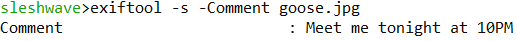
\includegraphics[width=8cm,keepaspectratio]{pics/metadata_message_identified}
    \caption{Example of message hidden in a file in the metadata section}
    \label{MetadataMessageExample}
\end{figure}

\section{Unused space embedding} \label{Unused_Space_Chapter}
Usually most file formats and even internationally approved and used protocols such as the TCP/IP have unused bits or bytes in their composition, either for future proofing the format in the form of reserved space or simply to serve as padding space mainly present to help the associated parsers. 

One well known example of this is found in the BMP file format which appears only in the cases where the width of the image is not a multiple of 4. The standards specify that in this situation there needs to be added the right amount of bytes to fill so that the width will be divisible by 4. So if an image has a resolution of 1920x1080 (the width is the first number), there won't be a need for any padding bytes because 

\[1920 \% 4 = 0\]

On the other hand, if the image had a resolution of 125x100, we would instead have

\[125 \% 4 \neq 0 \implies 4 - (125 \% 4) = 4 - 1 = 3\ bytes\]

to serve as a padding for each pixel line, ending up in a total of $100 * 3 = 300$ bytes of simple, raw, unused space that most BMP parsers will ignore because they know that data is meaningless. 

Another very good example is in the case of the IPv4 packet header which has a reserved bit in the flags subsection, or to be more precise, the 49th bit. According to RFC3514\cite{RFC3514} it is meant to be a security bit representing the true intent of the packet (GOOD or EVIL), however it is important to note that it was an April Fools informational memo and it is most likely that altering this bit will still go undetected by any kind of firewall or intrusion prevention system.

\begin{figure}[H]
    \centering
    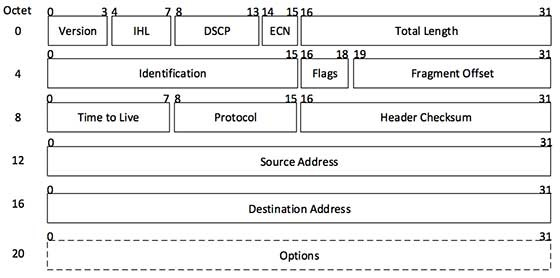
\includegraphics[width=8cm,keepaspectratio]{pics/ip_packet_specifier}
    \caption{The structure of an IP packet}
    \label{IP_Packet_Specifier}
\end{figure}

Given the IP packet header specifier represented in Figure \ref{IP_Packet_Specifier} it becomes trivial to alter the first bit of the flags section to the current bit of a secret and then over multiple sent packets to actually send the message in one of the most covert ways possible. Furthermore, it is very important to note the contribution done by Kamran Ahsan and Deepa Kundur in their 2002 article entitled "Practical Data Hiding in TCP/IP"\cite{practical_data_hiding_tcp_ip} because they also achieve the ability to send covert information by taking it one step further: using IP packet headers that may actually even be in use and by using Chaos Theory in the values of the Identification field sent over.

However, there is still one very important spot left in a file's byte stream where the secret message could easily be hidden: at the end of it. Most file formats either have specially crafted headers that announce the end of the file\footnote{One good example is the PNG format which has an IEND header and a couple of other information to mark that the image data has ended and that there is nothing left that is relevant to the parser. More information regarding this format is available in chapter \ref{BMP_Explained_Chapter}.} or have a few bytes reserved at the beginning of the file that mark the length of the data\footnote{This method is found in BMP or WAV file formats usually, it is very simple and easy to work with for parsers. More details in later chapters.}. It is important to note that both of these methods basically produce the same result technically speaking: a superior margin, a maximum amount of bytes that are to be read and interpreted by the parsers that contain the data relevant to the current file. After that region has ended, it is a free-for-all memory territory for secrets to be embedded. The same limitations from the previous chapter still stand, it is recommended that $MMS \leq  50\% * CDS$ in order to remain as covert as possible while still exfiltrating data.

\begin{figure}[H]
    \centering
    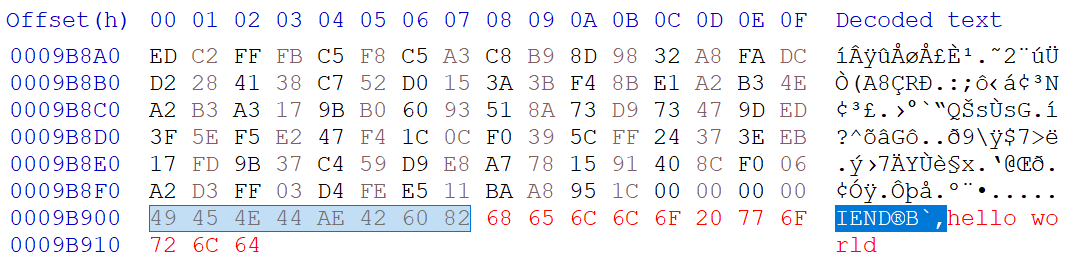
\includegraphics[width=9cm,keepaspectratio]{pics/secret_after_file_ended}
    \caption{Simple example of hiding a note after a file has ended}
    \label{secret_after_file_ended}
\end{figure}



\end{multicols*}

\chapter{Image file formats and steganography techniques}

\section{Introduction}

\setlength\columnsep{20pt}
\begin{multicols}{2}
An image is a two-dimensional representation depicting any possible subject conceivable by human imagination, captured using an optical device (such as a camera or a telescope) or a natural object (human eyes). The image can then be rendered and displayed for other people to see either manually (by painting, carving etc.) or automatically (by using a computer). In this chapter we will focus on images captured using digital optical devices that are rendered automatically. The correct term for them is digital images, but throughout the rest of the paper they will be reffered to as images for convenience.

\begin{figure}[H]
    \centering
    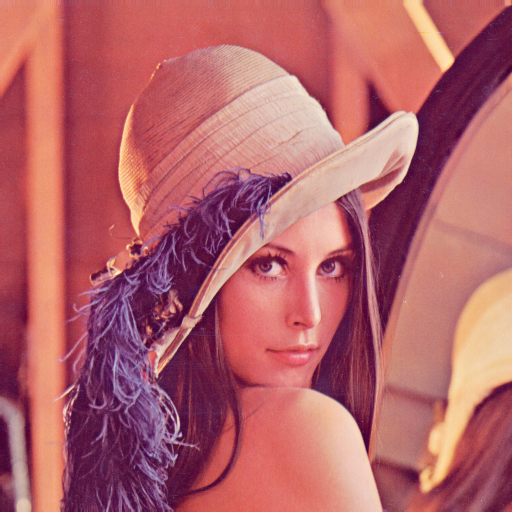
\includegraphics[width=5cm,height=5cm,keepaspectratio]{pics/lenna}
    \caption{Lenna - Classic example of a digital image}
    \label{Lenna}
\end{figure}

Computers are programmed to do operations in a clear sequential way and this rule doesn't change when working with pictures. In order for a computer to be able to render an image, it needs to know some general metadata information about the photo, such as the width and height, as well as the data bytes of the image. These bytes are the actual representation of the picture which compose the two-dimensional pixel map\footnote{This is true for a lossless format, where each pixel is stored in memory. It is not exactly the case for lossy formats such as JPEG where the image goes through processing before being rendered. More information later in the chapter.}. A pixel is the smallest unit that a computer monitor can read and display. The pixel color is the result of merging the different color channels which compose the picture (such as RGB, YUV, YCbCr etc.). Here is an example of the entire process - let's assume that from the image data bytes the first 3 bytes have the decimal values 20, 127, 250 and that it uses the RGB color model. This means that when the computer will have to render the image, the first pixel will have the red component equal to 20 (0x14), the green equal to 127 (0x7F), and the blue equal to 250 (0xFA), in what will finally be interpreted as \#147FFA by the monitor (variation of light blue). 

\begin{figure}[H]
    \centering
    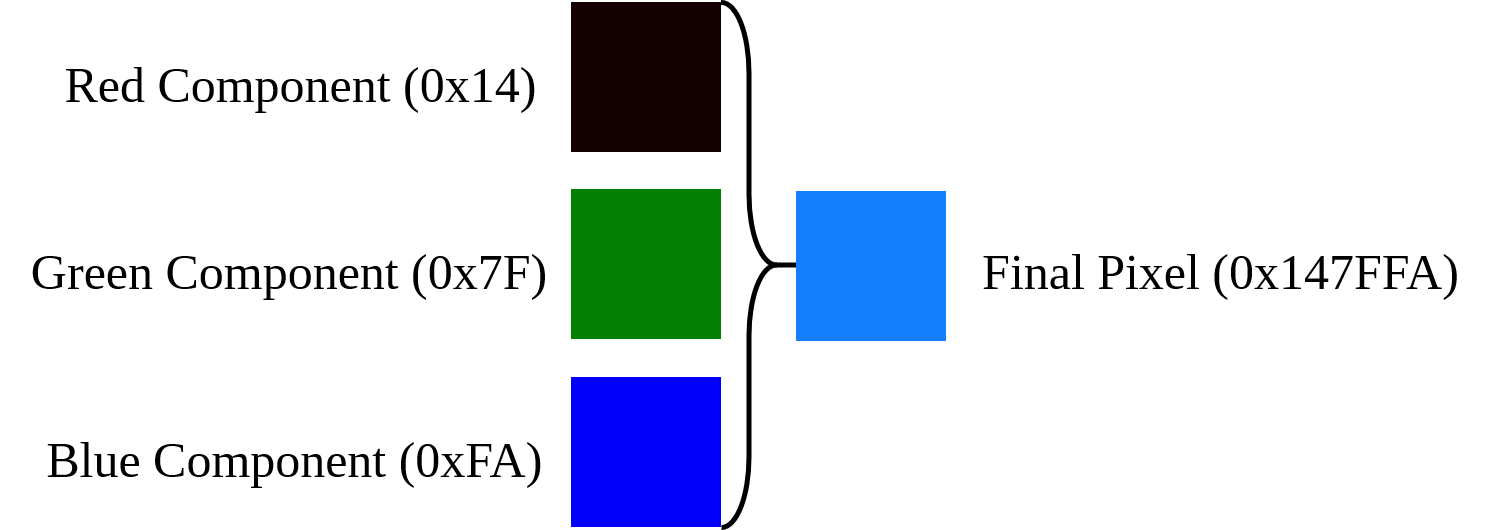
\includegraphics[width=8cm,height=2.15cm,keepaspectratio]{pics/how_a_pixel_works}
    \caption{How 3 colors channels build the pixel}
    \label{Pixel Creation}
\end{figure}

By merging multiple pixels over a two-dimensional space, they will eventually start to resemble an image that can be stored on a disk as a byte stream and can be rendered anytime by parsing the aforementioned stream. Each pixel can be represented as a point in that space with coordinates that are part of the unsigned integer domain. An entire row of pixels, i.e. pixels that have the same ordinate value, is sometimes also referred to as a scanline because in the earlier days of modern computing, computers would be given the width of the image and based on that value they would read a precise amount of bytes and render it on the screen before moving on to the next scanline, repeating this process until there would be no more information.

It is important to note that most of these developments have been done in a time where the maximum storage was extremely limited and not very fast, very different from what it is today. In order to save some space they looked into different compression algorithms to apply to the byte streams and today they fall into two distinict categories: the lossless algorithms are the ones that compress all the original information without destroying any of it, while on the other hand there are the lossy algorithms which are able to identify which information is useless and delete it accordingly. This concept also applies to file formats and we will see in later chapters more concrete examples. 

With all of this information in mind, we can now procede to discussing the most commonly formats commonly used in today's.

\section{BitMap Picture (BMP)} \label{BMP_Explained_Chapter}

The BMP file format, also known as the device independent bitmap file format(DIB), bitmap image file or just bitmap, is a lossless\footnote{It is true that the format specification standards supports compression but further research reveals that currently it only supports lossless types of compression, such as the Huffman or Run Length Encoding algorithms.} image file format originally designed by Microsoft back in 1986 in order to store two-dimensional digital images on their Windows operating system. Over the years it has developed plenty of variations and extensions that were based on the original specification but this paper will focus only on the most common available ones, no extended versions that are looking to improve the format since they do not add anything interesting or new to the way the format stores the data thus affecting the steganography algorithms.

As with almost every file format, the final BMP byte stream can be seen as a result of the merge between the BMP header which contains metadata about the file and the BMP data which is the actual pixel information. As we can see from table \ref{BMP_Header_Table}, the BMP header stores a lot of important information about the image that is useful for any rendering software while making sure to allocate enough memory to be able to display the picture on the screen and other essential steps. It is also important to note that all the structures seen in the BMP header use the little-endian format for representation and are usually more troublesome on the systems that have the default set as big-endian.
\end{multicols}

 \begin{center}
	\begin{tabular}{|l|l|l|l|}
		\hline
		\textbf{Information} & \textbf{Size} & \textbf{Offset} & \textbf{Description} \\ \hline
		Signature & 2 bytes & 0x00 & Two chars, 'B' and 'M' \\ \hline
		File size & 4 bytes & 0x02 & Total file size in bytes \\ \hline
		Reserved & 4 bytes & 0x06 & Unused space \\ \hline
		Data offset & 4 bytes & 0x0A & Offset to get to the actual BMP data \\ \hline
		Size & 4 bytes & 0x0E & Size of the left header information \\ \hline
		Width & 4 bytes & 0x12 & Horizontal size of the image \\ \hline
		Height & 4 bytes & 0x16 & Vertical size of the image \\ \hline
		Planes & 2 bytes & 0x1A & Amount of image planes \\ \hline
		Bits Per Pixel & 2 bytes & 0x1C & How many bits are used to represent each pixel \\ \hline
		Compression & 4 bytes & 0x1E & Indicates the type of compression used \\ \hline
		Image size & 4 bytes & 0x22 & The size of the compressed image, can be 0 \\ \hline
		X pixels per Meter & 4 bytes & 0x26 & Horizontal resolution in pixels/meter \\ \hline
		Y pixels Per Meter & 4 bytes & 0x2A & Vertical resolution in pixels/meter \\ \hline
		Colors Used & 4 bytes & 0x2E & \begin{tabular}[c]{@{}l@{}}Number of actually used colors\\ (based on Bits Per Pixel)\end{tabular} \\ \hline
		Important Colors & 4 bytes & 0x32 & Number of important colors (usually all) \\ \hline
	\end{tabular}
	\label{BMP_Header_Table}
 \end{center}

\begin{multicols}{2}
Analyzing the obligatory BMP header fields we realise that most of them are useless for any steganographic purposes mainly because they can't be altered without having major consequences on the renderer software but there are still a few interesting ones left:
\begin{itemize}
  \item The 4 bytes that are reserved and unused could be very well put to use by using the methods presented in chapter \ref{Unused_Space_Chapter}, so we can use either this space to send parts of a message over multiple BMP files, or we can store the secret message size in these 4 bytes and write the secret after the actual image data has ended.
  \item Data offset could be useful because some renderers use this field to indicate the offset of the actual image data and just skip any other irelevant metadata information, allowing us to hide information in those fields.
  \item The width and the height of the image usually are altered to hide bottom parts of the image that may contain hidden information or by masking the result of the merge of two images and just showing the top one. Let's take for example this image of the sun that is obviously missing a part for demonstration purposes.

\begin{figure}[H]
    \centering
    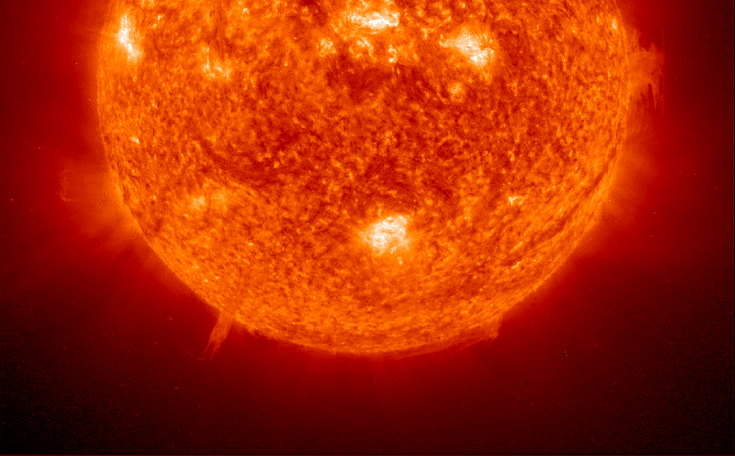
\includegraphics[width=4cm,keepaspectratio]{pics/height_modification_steganography_cut}
    \caption{Incomplete sun image}
    \label{Sun_Missing_Part}
\end{figure}

However if we adjust by trial and error the height of the image to see if there is any more bytes to render, we would notice that there really is a message hidden with those bytes that some steganalysis softwares would detect but any renderer software such as the Windows Media Viewer would always miss. In other words, we have tricked the software to not display more scanlines than we wanted it to display, even though the information is there, not corrupted in any way.

\begin{figure}[H]
    \centering
    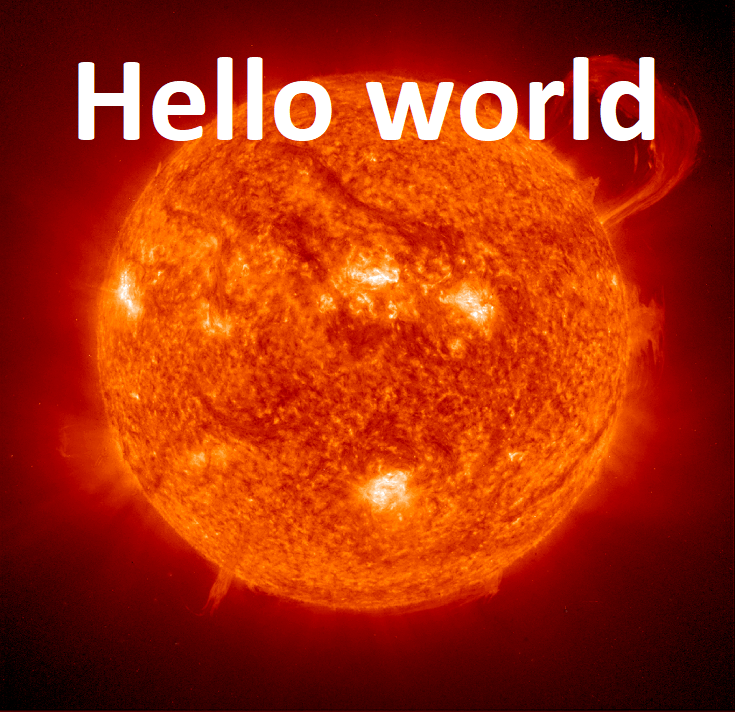
\includegraphics[width=4cm,keepaspectratio]{pics/height_modification_steganography_original}
    \caption{Complete sun including the hidden message}
    \label{Sun_Original}
\end{figure}
\end{itemize}

Moving on from the metadata block of the BMP format to the actual data byte stream, we find additional interesting information about how the pixel data is actually stored. Most images use the Red, Green and Blue also known as RGB values to compose the final pixel color, but for an unknown reason the creators of the bitmap format decided to store the information in the reverse order in the data stream as Blue, Green, Red or BGR. However this is not the only change they made from the other common image formats available at the time: rather than storing the scanlines from a top to down order, BMP decided to store them bottom-up.

\begin{figure}[H]
    \centering
    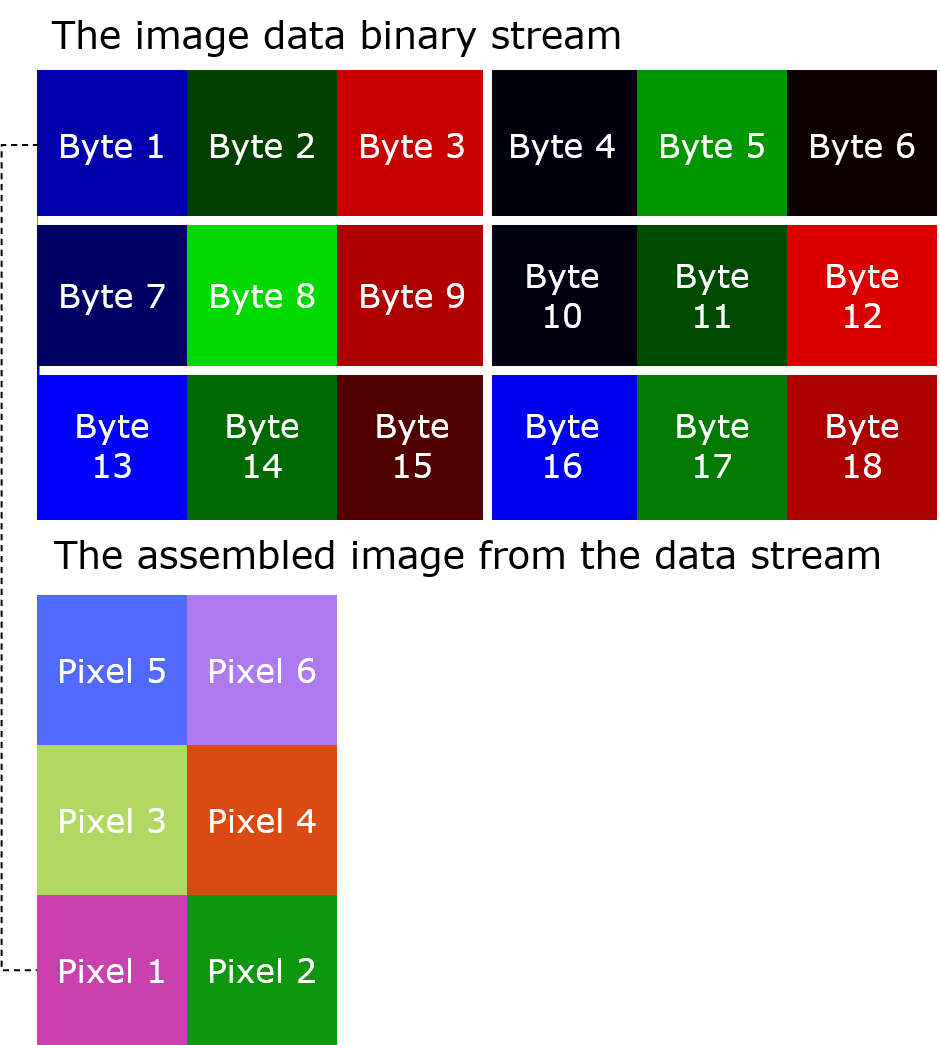
\includegraphics[width=7cm,keepaspectratio]{pics/assembling_bmp_image}
    \caption{How the BMP image is rendered}
    \label{bmp_how_to_render}
\end{figure}

This behaviour can be noticed in figures \ref{Sun_Missing_Part} and \ref{Sun_Original} where the top part is cropped in order to hide a message and we can now understand why it is only that part that can be made redundant in the steganography process: because the last bytes of the image data binary stream are actually responsible for the rendering of the top section of the picture. Seeing and understanding how the carrier format works is the first and most important step in embedding messages in a covert way.

\subsection{Image sub-block scrambling using the BMP format}
Sub-block scrambling is a type of scrambling algorithm, like those introduced in chapter \ref{scrambling_chapter}, that can be applied to images stored in the BMP format. It was created by the author of this thesis based on the idea of the JPEG format and the algorithm it uses during compression that is applied only on sub-blocks of 8x8 size. We mentioned in chapter \ref{scrambling_chapter} that most scrambling algorithms have \[ MMS \leq [CDS \ / \ 8] \ bytes \] but the target was to design and implement an algorithm which can make use of all the bytes available in the cover, and we ended up with this method which has 
\begin{equation} \label{eq:1}
MMS = [CDS \ / \ 8] \ bytes
\end{equation}
 making it similar in storage capacity to a sequential algorithm. That performance was achieved following a simple procedure:
\begin{itemize}
  \item Separate the image into multiple blocks of BLOCK\_SIZE (this is a global constant value which is usually equal to 8 but can be higher or lower). It doesn't matter if the width or height of the image are not a multiple of BLOCK\_SIZE, the algorithm also works with non-square blocks.
  \item The algorithm needs a password to work with in order to use it as a seed when generating a permutation. Each block calls a helper method to obtain the given permutation for itself based on its own width and height. That permutation is the order in which the data will be written.
  \item The first block is reserved for writing the metadata about the message(such as the length of the secret) and the other blocks are for writing the actual contents of the message.
\end{itemize}

\end{multicols}

\definecolor{lightergray}{rgb}{0.92,0.92,0.92}
\lstset{escapeinside={<@}{@>},
		frame=single,
		xleftmargin=-25.4pt,
	      xrightmargin=-25.4pt
}

\begin{lstlisting}[backgroundcolor = \color{lightergray},language=Python,caption={Pseudocode of the scramble algorithm},captionpos=b,label=lst:scramble_pseudocode]
 global constant BLOCK_SIZE;

 procedure embed_subblock(secret, subblock, random_engine)
   #Generate a permutation from 0 to subblock.width * subblock.height
   #using the random_engine given. That permutation will be the order
   #used when writing the secret data into the subblock data.
   writing_order<@$\gets$@>random_permutation(0,subblock.width*subblock.height,random_engine); 

   for each byte_index in writing_order do
     #Getting the absolute index of the subblock rows and 
     #columns where we need to write the secret information.
     subblock_row<@$\gets$@>subblock.starting_line_index+byte_index/subblock.width;
     subblock_column<@$\gets$@>subblock.starting_column_index+byte_index%subblock.width;
     set_least_significant_bit(subblock.data[subblock_row][subblock_column],secret);

     #We move to the next bit of the secret information
     advance_to_next_secret_bit(secret);
		
 procedure pseudo_scramble(cover, secret, password)
   #Creating a new pseudo-random engine with a given seed.
   random_engine<@$\gets$@>new pseudo_random_engine(password);

   for each subblock of cover with subblock.size<@$\leq$@>BLOCK_SIZE
     if subblock = cover.first_subblock
       #Used for hiding the size of the secret into 
       #the first subblock of the cover in an order
       #given by the pseudo-random engine random_engine.
       embed_subblock(secret.size,subblock,random_engine);
     else
       #If it's not the first subblock of the cover, 
       #write the actual secret into the subblock.
       embed_subblock(secret.iterator,subblock,random_engine);

\end{lstlisting}

\begin{multicols*}{2}
It is much easier to explain the algorithm using a simple example, so let's begin with the image represented in figure \ref{scramble_example_original_image}. It is BMP image with a resolution of 10x6 pixels (10 pixels wide, 6 pixels tall). Furthermore, let's also create the parameters needed by the algorithm in order to embed a message:
\begin{itemize}
  \item The secret message we want to hide in the cover file is "Hello World", no quotes.
  \item Given the aforementioned message, we can calculate its size: 5 characters for the word "Hello", 5 characters for "world" and 1 character for the space inbetween. Total message length is 11 characters or 11 bytes using the ASCII standard. 
  \item The password used for generating the seed is "super\_secret\_key", no quotes.
  \item The BLOCK\_SIZE used in splitting the original image is equal to 4.
\end{itemize}

\begin{figure}[H]
    \centering
    
\includegraphics[width=7cm,keepaspectratio]{pics/bmp_scrambling/original_image}
    \caption{Original BMP cover image}
    \label{scramble_example_original_image}
\end{figure}

Knowing all of this information we can already know if the cover file is going to be able to hold the secret message based on the formula \ref{eq:1}. We know that the BMP format uses 3 bytes for storing each pixel and that our image is 10 pixels wide and 6 pixels tall, so we have that 
\\$CDS=3*10*6=180\ bytes \overset{(\ref{eq:1})}{ \implies }\\ \overset{(\ref{eq:1})}{ \implies } MMS=[180/8]=22\ bytes$

Since our total message length is smaller than $MMS$, we know that we will not be running out of cover space during the embedding process. After making these verifications, we can begin by initializing our pseudo-random engine based on the given password meant to be used as a seed and we can also start splitting the original image into sub-blocks, ending up with a result similar to figure \ref{scramble_example_subblocks}. Since neither the width or height of the image are multiples of the BLOCK\_SIZE constant, we have several smaller blocks (to be more precise, blocks 3, 4, 5 and 6) that are still going to be used for embedding purposes. 

\begin{figure}[H]
    \centering
    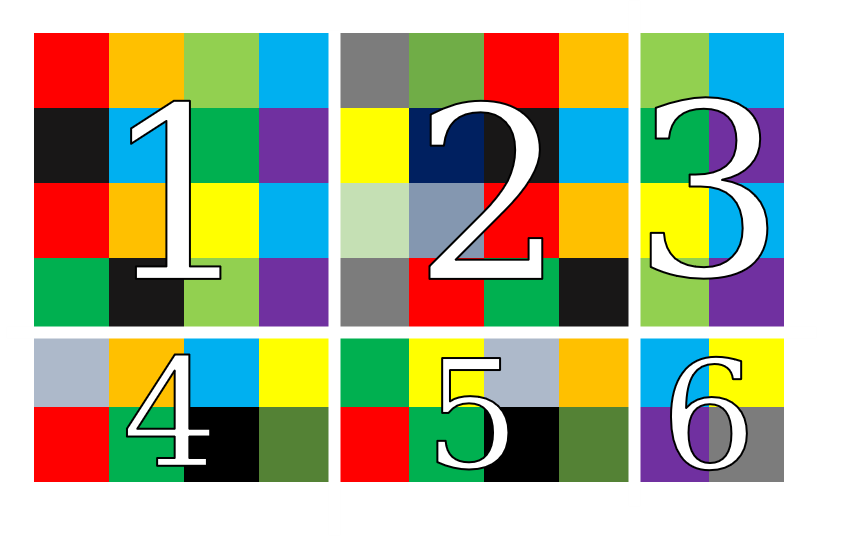
\includegraphics[width=7cm,keepaspectratio]{pics/bmp_scrambling/image_broken_subblocks}
    \caption{Sub-blocks of the original image}
    \label{scramble_example_subblocks}
\end{figure}

We can now begin the actual embedding process. From the pseudocode presented in listing \ref{lst:scramble_pseudocode} we see that the first step is to embed metadata about the secret message, more specifically its length represented as an unsigned integer on 32 bits. But before we can do that, we must ask the pseudo-random engine to generate a permutation between 0 and $subblock.width * subblock.height$, excluding the last value. For this example specifically, we know that
\[ subblock.width * subblock.height = 4 * 4 = 16 \]
and let's assume that the engine returns us the following permutation: 
\[(5,10,12,3,0,15,4,9,14,13,8,2,7,1,6,11) \]
With this order known and with the fact that each BMP pixel is represented on 3 bytes giving us 3 least significant bits for embedding purposes in mind, the process of embedding the message length (11 or 0x0000000B) into the first subblock goes as follows:
\begin{enumerate}
  \item 5th pixel is the first one, all LSBs are set to 0.
  \item 10th pixel, all 3 LSBs are set to 0.
  \item 12th pixel, all 3 LSBs are set to 0.
  \item 3rd pixel, all 3 LSBs are set to 0.
  \item 0th pixel, all 3 LSBs are set to 0.
  \item 15th pixel, all 3 LSBs are set to 0.
  \item 4th pixel, all 3 LSBs are set to 0.
  \item 9th pixel, all 3 LSBs are set to 0.
  \item 14th pixel, all 3 LSBs are set to 0.
  \item 13th pixel has the Blue channel LSB set to 0, Green channel LSB set to 1, Red channel LSB set to 0.
  \item 8th pixel has the Blue channel LSB set to 1, Green channel LSB set to 1, Red channel is unchanged.
  \item The rest of the pixels are unchanged.
\end{enumerate}

A visual representation of the order based on the given permutation can be found in figure \ref{scramble_example_first_block}. We can also notice that we managed to embed 4 bytes of information into a simple block of 4x4 pixels, or 48 bytes of total data, and we still have 2 bytes of free space based on \ref{eq:1}(one bit available in 8th pixel and 3 bits in pixels 2,7,1,6,11).

\begin{figure}[H]
    \centering
    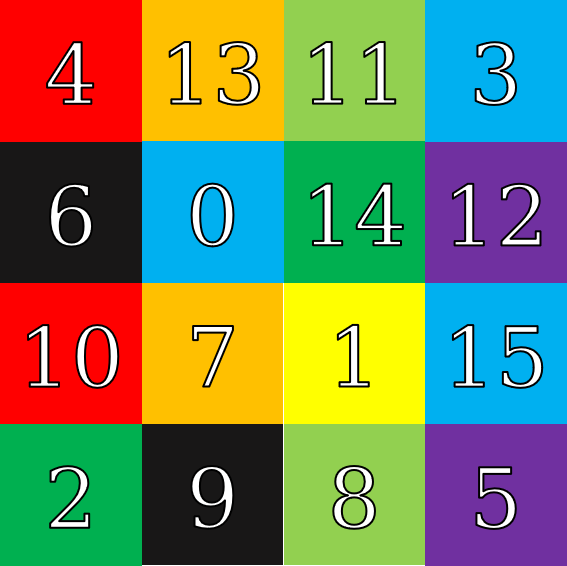
\includegraphics[width=5cm,keepaspectratio]{pics/bmp_scrambling/first_block_marked}
    \caption{Order of writing into the first block}
    \label{scramble_example_first_block}
\end{figure}

After embedding the metadata, we can begin hiding the actual message data into the subblock bytes. The sub-block size is 4*4 pixels total, which means 48 bytes in total space, resulting in exactly 6 bytes we will be able to write into this subblock (and every other block which uses 3 bytes to store a pixel and has 16 pixels in total). We start by converting our secret message in binary and we end up with something like this:
\begin{enumerate}
\item H = 01001000
\item e = 01100101
\item l = 01101100
\item l = 01101100
\item o = 01101111
\item (space) = 00100000 
\item w = 01110111 
\item o = 01101111 
\item r = 01110010 
\item l = 01101100 
\item d = 01100100
\end{enumerate}
By knowing we have 6 bytes available in the first sub-block we will be able to hide the string "Hello ", which is impressive because it is already more than half of our total message in an image that is only 4 pixels wide and 4 pixels tall. Before starting the actual embedding process, we must again use the pseudo-random engine to generate a new permutation ranging from 0 to the total amount of pixels in the block. Again for the sake of our example, let's assume that we get this permutation:
\[(10,4,12,6,1,15,9,3,0,8,13,5,2,14,7,11)\]
Using the binary conversion of our message, we begin by taking 3 bits each time from the binary stream and embedding them into each channel of a pixel in the order given by the permutation. We can see what bits we have written into which pixels in figure \ref{scramble_example_second_block} (the first bit is the one written into the Blue channel of the pixel, the middle one is the Green channel and the last bit is encoded into the Red channel).

\begin{figure}[H]
    \centering
    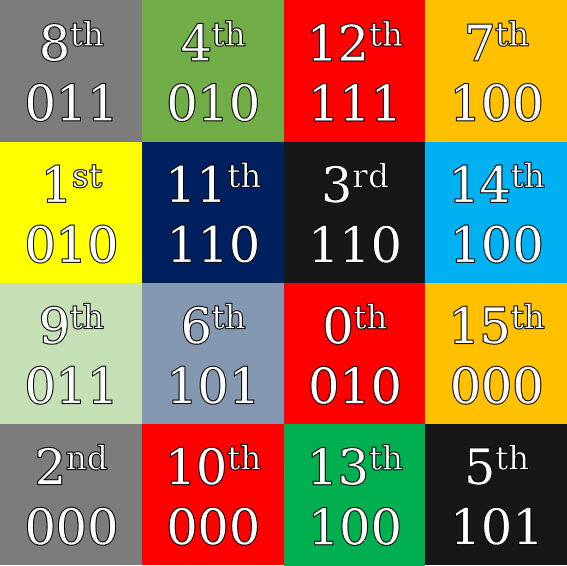
\includegraphics[width=6cm,keepaspectratio]{pics/bmp_scrambling/second_block_marked}
    \caption{Order of writing the actual message into the second block}
    \label{scramble_example_second_block}
\end{figure}

In the case of the third block the situation is slightly different because the width of the block is not equal to BLOCK\_SIZE but this change does not change the behaviour of the algorithm at all. In this case we have a block that is 2 pixels wide and 4 pixels tall, ending up with a total of total 24 bytes needed for storage that can accomodate 3 bytes of secret information, or in our case the letters 'w', 'o' and 'r'. In this case we generate a permutation from 0 to 8, excluding the last value:
\[(3,6,0,1,4,7,2,5)\]
By going through the same process as with the previous block we get the result that can be seen in figure \ref{scramble_example_third_block}. This leaves us with the target of hiding only two more characters: 'l' and 'd' in block number 4 which is identical to block 3 in size but was rotated by 90 degrees. 

\begin{figure}[H]
    \centering
    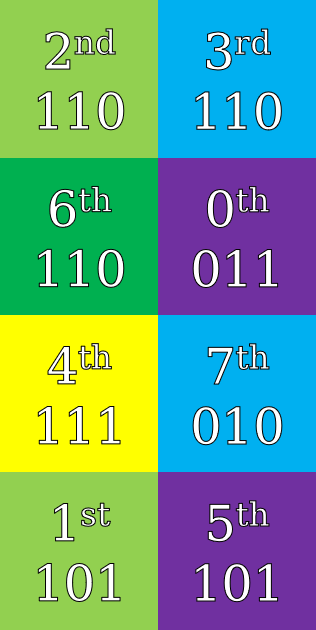
\includegraphics[height=5cm,keepaspectratio]{pics/bmp_scrambling/third_block_marked}
    \caption{Order of writing into the third block}
    \label{scramble_example_third_block}
\end{figure}

For the last time we generate a permutation using the engine in the same interval as above and we obtain:
\[(5,3,0,7,4,2,6,1)\]
And by going again through the steps described above we manage to hide the last two remaining characters and we still have a byte free in the sub-block. The remaining blocks of the image remain unchanged and theoretically could be used for hiding other messages, but there are a few issues that can arise with this, the main one being message separation and identification, how each message is divided etc.

\begin{figure}[H]
    \centering
    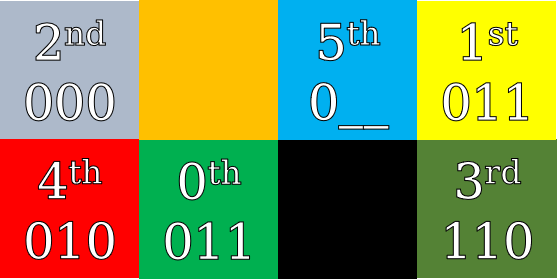
\includegraphics[width=5cm,keepaspectratio]{pics/bmp_scrambling/fourth_block_marked}
    \caption{Writing the actual message into the fourth block}
\end{figure}

After the algorithm finishes and the modified cover image is saved, there is absolutely no difference to the human eye between the two pictures. This is the power of Least Significant Bit insertion when using digital images as the carrier format. The only difference between the two files is at a bit level, making it one of the safest and most covert ways of sending secrets over an untrusted environment.

\begin{figure}[H]
    \centering
    
\includegraphics[width=5cm,keepaspectratio]{pics/bmp_scrambling/original_image}
    \caption{The original image}
\end{figure}

\begin{figure}[H]
    \centering
    
\includegraphics[width=5cm,keepaspectratio]{pics/bmp_scrambling/altered_image}
    \caption{The altered image containing the message "Hello world"}
\end{figure}

Like any other steganography algorithm, this method also has advantages and disadvantages. The main benefits of this algorithm are:
\begin{itemize}
  \item \textbf{Security}. Choosing a BLOCK\_SIZE of only 8, each normal sized block will have a total of 64 pixels and there would be $64! = 1.2688693e+89$ ways available (just for a single block) for the algorithm to write the secret information. Given the fact that each block has its own permutation generated specifically for it based on a pseudo-random engine makes it very hard for any intruders to try and retrieve the secret message without having access to the key. Increasing the size of the BLOCK\_SIZE only strengthens the overall security of the method while still keeping the same message capacity.
 \item \textbf{Efficiency}. The algorithm is extremely fast because it performs very few demanding operations and it is taking advantage of bit-wise operations. Furthermore, there is also the option of adding parallelization because there are no conflicts whatsoever between the parties involved, thus ending in an even more efficiency increase for the entire operation. There could be a small issue regarding the generation of the permutations based on a key in a multi-threaded environment because it may be prone to some implementation language issues with the pseudo-random engine.
\end{itemize}
However there are quite a few issues with this algorithm, issues that can render the method useless and make it obsolete in a faster than normal timeframe:
\begin{itemize}
  \item \textbf{No data redundancy}. There is absolutely no mechanism in place in order to prevent the loss of data. Most communication environments nowadays usually compress the files before sending them over the wire and that compression may be lossless, but in most cases it is lossy. And even by sending the file in a way that it will not be compressed, there is also the slight change of altering and a small change in a single bit can and it will make the whole secret message corrupted without any method of recovery.
  \item \textbf{Detection via pattern identification}. Working only within small sub-blocks of BLOCK\_SIZE means that we also limit the attack surface of any outside parties and allow them to focus on finding any details that can help them identify the key that was used when encoding the secret. For example, it is possible that an attacker will want to focus on the second block of the cover file and try to search for common extensions in the secret embedded file headers. If the intruder finds there is an order to the bytes of the block which produce that header that means that he is much closer to identifying the seed of the pseudo-random engine because he knows the second permutation generated by that seed and based on that information he may be able to deduct further permutations.
  \item \textbf{Limited market}. This algorithm was designed with file formats that are lossless, i.e. bitmaps that store the entire information of the image. While theoretically it could be used for PNGs as well, we will see in later chapters that PNG uses a mechanism called interlacing which makes it harder to work or even identify the sub-blocks of the image. Most modern online platforms have also moved away from BMP since they are far too big in size and the same image quality could be achieved by using other formats that have a much much smaller size, ending up in almost making the entire BMP format obsolete.
\end{itemize}
In the end, it is important to note that similar work has been done by a few researchers, the closest one being the work done by Hussein Al-Bahadili\cite{secure_block_permutation} in his paper where he chose to focus on scrambling the contents of the secret message using a similar password and seed generation technique before writing it to the carrier file. But while the 2 methods are similar in their goal, the way they reach that goal are different.


\section{Portable Network Graphics (PNG)} \label{PNG_Explained_Chapter}


\end{multicols*}


\chapter{Audio file formats and steganography techniques}

\begin{multicols}{2}
\section{Introduction}
Sound is the result of a vibration created by a phenomenon that propagates through a transmission environment, ending up getting interpreted by our brain. However since this process happens in the physical world it is entirely analog so it would be impossible to store it on modern day devices which can only understand digital formats. Luckily the fast evolution of computers also brought conversion techniques in order to switch between analog sounds and digital sounds seamlessly, without any noticeable loss to the human ear. Using these methods we have gained the ability to store audio files in a digital format so it was only logical that several different file formats will be created to fit our needs. In this chapter we will discuss in greater detail about how the analog data is actually stored in the digital format and what are the most common extensions used for storing digital audio files.

We mentioned earlier that it is impossible to store analog signals in a digital environment. The solution to this problem is to convert the audio signal which can be represented as a continuous-time function into a discrete-time function using a process called sampling. 

\begin{figure}[H]
    \centering
    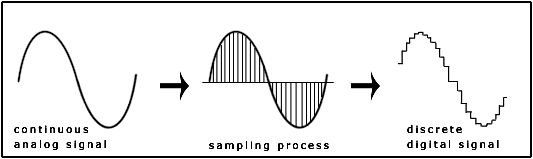
\includegraphics[width=7.7cm,keepaspectratio]{pics/Sampling-of-audio-signal.png}
    \caption{Converting a continuous signal into a discrete one\cite{real_time_audio_steganography}.}
    \label{sampling-graphic-example}
\end{figure}

The sampling process can be observed in figure \ref{sampling-graphic-example}. We can now introduce some new terms that we will use throughout the rest of the chapter:
\begin{itemize}
	\item \textbf{Sampling rate} is the number of samples taken per second, or in other terms, how many discrete values we store for each second of the audio signal. The measurement unit for sampling rate is Hertz (Hz for short) and some of the most common values are 44100, 48000 and some of their multiples.
	\item \textbf{Bit depth} is the number of bits used to store a single sample after having it converted to a discrete value. The most common bit depths are 8, 16, and 24 which allow for 256, 65536, and 16777216 different values. 
	\item \textbf{Audio channel} is the term used to describe the sequence of bytes that represent sampled audio signals. An audio file can have multiple channels to better simulate the sound accuracy and origin in a limited environment. Files with one audio channel are called mono, with two they become stereo and any more channels makes them surround. However, no matter the number of channels, usually all of them are equal in length and the samples from each channel are played simultaneously.
\end{itemize}

In the steganography field, the most common configuration that accepts alterations to the sampled data without losing any noticeable quality is a sampling rate of 44.1kHz with a bit depth of 16 and any number of audio channels, so this the ideal format that we will use throughout the rest of the chapter. The reason why this configuration is favored so much is because of the popularity that came with the invention of CDs and MP3s which used it as a default. Furthermore, any changes made to the sampled data are usually small enough that they will not be noticeable according to the Nyquist-Shannon sampling theorem \cite{Shannon1949}, which is used to compute the condition such that the conversion from a continuous signal to a discrete one will capture all the relevant information. Using the aforementioned theorem and armed with the knowledge that the human physiology enables us to hear audio signals ranging from 20Hz to 20kHz, we can see why the 44.1kHz sampling rate is ideal in audio steganography.

\section{Additional techniques used in audio steganography}
\subsection{Frequency domain steganography}
So far in this thesis we have talked about what can only be classified as spatial domain steganography, like how a pixel of an image is composed of bytes and that altering those byte values in a smart way allows for message embedding or how we can use the file specifications to our advantage and hide information in the file metadata or after the offset where all renderer programs will stop parsing. All of the previous examples deal ony with the spatial domain of the format because they work on the raw bytes and consider each of them to be completely individual and self-sustaining entities that can be altered for steganographic purposes. However, there is another domain that works differently than the spatial one and it is called the frequency domain. In this domain the final representation of the stored data is done by combining the entire range of frequencies into the equivalent signal, usually by using a transform function, the most common being the Fourier transform. The advantage of the frequency domain is that it helps split a signal of any type into clear and distinct sinusoids that are easier to perform complex tasks on. 

In figure \ref{time_vs_frequency_comparison} we can see the differences between the time domain and the frequency domain: the former evolves over time and is highly irregular in most cases(in real world there will never be a perfect sinusoidal signal and will be more similar to the last example), while the latter is easier to manipulate and identify, and through the aforementioned transform functions can be converted back into the time domain.
\begin{figure}[H]
    \centering
    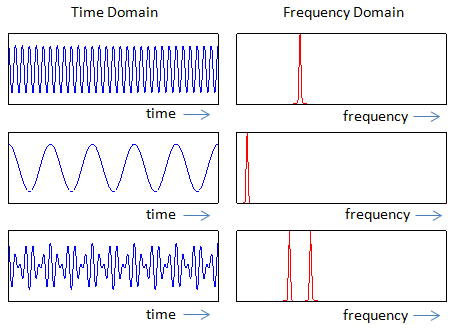
\includegraphics[width=7.7cm,keepaspectratio]{pics/audio_chapter/time_vs_frequency_domains.png}
    \caption{Time domain vs. frequency domain.}
    \label{time_vs_frequency_comparison}
\end{figure}

In the digital images world, the frequency domain is used to know by how much pixels variate from one another, in other words, the rate with which the pixels change. The most common format used for images that takes advantage of the frequency domain is JPEG, but since it is the only known format which uses sinusoids when rendering the image, the authors chose not to include it since the steganographic surface was somewhat limited. However, in the digital audio world every sound will eventually become an analog signal before reaching our ears so it is more common to see algorithms developed specifically for this format that involve altering the sinusoids to our advantage.

For example, we have the technique described in the article Frequency Domain Steganography by Ganier et al.\cite{ganier_hollman_rosser_swanson} where they showcase the most basic way of embedding an audio file within another audio file: since both files have audio signals that are stored as frequencies, it is possible to "compress" the signals so that they only occupy a very specific frequency range and hide the message within the inaudible frequencies of the carrier, a much trivial task when not working in the time domain. This method takes advantage of the human physiology we mentioned earlier and achieves a high rate of success. Similar work has been done by Westfeld et al. \cite{dsss_sstv} where they took the audio signal generated by the Slow Scan Television(SSTV) and embedded it into another carrier audio signal without any audible noise being generated that could alert intruders. On the more technical and software side of things there are applications such as Audacity that can integrate plugins written in a language called Nyquist that are specifically designed for frequency encoding secret messages, along with Matlab implementations of the aforementioned papers and many more.

Furthermore, there is also the option of steganography done within the spectrogram of a signal. A spectrogram is the visual represention of the entire spectrum of the frequencies as it evolves over time, basically getting the frequency domain and reintroducing the time axis into it. It is by far the most common place of hiding messages because it has been popularized by Capture the Flag competitions as entry level challengs and easter eggs in the video game community created by the developers. An example of hiding a key inside the spectrogram of an audio file can be seen in figure \ref{battlefield_spectrogram_easter_egg}, made by the developers at DICE for their community in a secret challenge\cite{battlefield wiki}.

\begin{figure}[H]
    \centering
    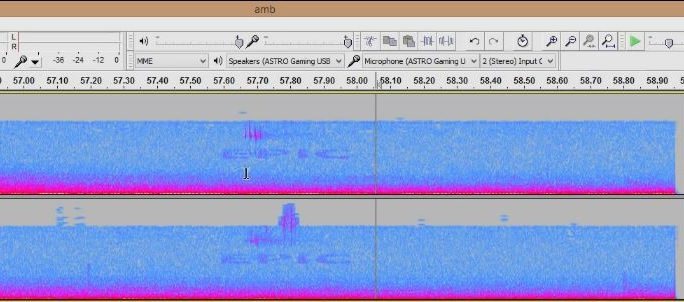
\includegraphics[width=7.7cm,keepaspectratio]{pics/audio_chapter/spectrogram_encoding.jpg}
    \caption{Message within the spectrogram viewed using Audacity.}
    \label{battlefield_spectrogram_easter_egg}
\end{figure}


\section{The MPEG-1/2 Audio Layer III (MP3)}
TO DO: research the MP3 format, how they store the audio samples, headers, compression, why it became so popular etc.

\section{Waveform Audio (WAV)}
The Waveform Audio format commonly known as WAV is a popular file format for storing high quality digital audio files originally built by Microsoft. It bears many similarities to the PNG format in the internal structure/composition of the file: both begin with a very specific sequence of bytes (also known as the magic bytes) that help classification applications identify them, are separated into multiple parts (also known as chunks) that have their purpose and are extremely common in the modern day multimedia.

TO DO: talk about the structure of the WAV format and the support for the steganography algorithms aforementioned.
\end{multicols}

\chapter{The Steganos Project}
\begin{multicols*}{2}
Steganos is the name of the application that implements the algorithms enumerated in the earlier chapters of this paper and is the direct result of the work done by the authors. In this chapter I will present what modern technologies and frameworks went into creating the application, how it is structured from an Object Oriented point of view, how fast it is and how I hope it will expand into the future.

\section{Used technologies}
\subsection{C++}
C++ is one of the lowest high-level computer programming languages. Designed by Bjarne Stroustrup, it first appeared in 1985 as a variation of one of the most popular languages at the time, C. It is one of the most efficient modern languages mainly because it has been designed with performance and flexibility in mind, just like its predecessor. C++ has gained a lot of traction  from big companies like Intel and Microsoft which needed a programming language that could be used for operations ranging from basic kernel functions to highly specialized Object-Oriented projects with Graphical User Interfaces\cite{stroustrup_2018}.

Since its conception, C++ has grew substantially by adding support for generic and functional features to ease the development processes and getting standardized by the International Organization for Standardization probably helped as well because it meant no more obscure variations of the language, allowing programmers to follow only one standard, ending up with even more portability and stability of the applications.

In the modern day, it is used almost everywhere: the kernel of various operating systems, the transaction software used by banks, drones and airplanes, embedded systems such as the Arduino or Raspberry Pi, and now in the Steganos Project as well under the latest approved standard of the language, C++17.

C++ inherited from C the file types: headers and sources. The header files (the files that have a .h or .hpp extension) are where the standard recommends to store the class declarations, function prototypes, constants declarations, no definitions should take place in a header file. There are a few exceptions to this rule, the most common one being a rule that states that all templated functions and functions are to be declared and defined in a header file otherwise it will not work properly when dealing with multiple instances of different types. In the case of the source files (the files that have the .c or .cpp extension) the standard suggests to only be used for the definition of the class methods or other general functions. Following the standard results most of the time in a clean and well defined separation in the code, allowing for high cohesion and low coupling in all projects built using C++.

The reason for choosing C++ as the language for the Steganos project is simple: it allows for the programmer to work on the raw bytes of files in an extremely easy way, reading and parsing them, bit-wise operations and writing to file, all the common low-level operations that are highly valued when working in the steganography field. But the high level aspects of the language also permit for dealing with complex tasks, such as modern cryptography algorithms applied to robust byte streams or holding all the information in different data structures.

\subsection{CMake}
CMake is a cross-platform open-source tool designed for managing the build process of software based on the C++ programming language. It has been created in the year 2000 and ever since then it stayed compiler-independent using simple configuration files that generate the adequate makefiles to be used in the users environment while building the target project\cite{cmake}.

CMake uses files called CMakeLists.txt that contain the commands to be used by the internals of the tool in the building process. It is required that one file is in the root of the project before running the CMake process, with the possibility of adding a .txt file in the subdirectories in order to indicate special cases that require a different approach.

\begin{figure}[H]
    \centering
    
\includegraphics[height=6.9cm,keepaspectratio]{pics/cmake_folder_structure_example}
    \caption{Folder structure of a project using CMake}
\end{figure}

Each command in CMake has the same format: COMMAND (args..). Using this format, users are able to build even the most complex software projects in the form of simple executables, dynamic or static linked libraries, etc. Steganos uses CMake because it is an extremely effective tool in the building process and it allows for separating the logic of the project into distinct modules i.e. the audio module, the image module, the general usage module, and linking them in the end into a simple executable. Most projects use only a small subset of the commands available in CMake, the most common being:

\begin{itemize}
  \item \textbf{CMAKE\_MINIMUM\_REQUIRED} is used to mark the minimum version of CMake that is required to be installed on a system in order to build the project.
  \item \textbf{SET} is used to assign a value to a CMake variable that is used while building, similar to environment variables found on all operating systems.
  \item \textbf{PROJECT} for naming the project, important step in active Continous Integration and Continous Development environments.
  \item \textbf{INCLUDE\_DIRECTORIES} for marking the directories containing the header files in order for the compiler to be able to link the source files and header files.
  \item \textbf{ADD\_EXECUTABLE} for creating an executable after build the project from the source files given as arguments.
  \item \textbf{ADD\_LIBRARY} for creating a library or module with the given source files.
  \item \textbf{TARGET\_LINK\_LIBRARIES} for linking (pre)defined modules or executables between eachother.
\end{itemize}


\subsection{CXXOpts}
CXXOpts is an open-source C++ library that is meant to be a lightweight command line option parser\cite{jarro2783_2020}. It is meant as the C++11 and beyond alternative to other libraries such as Commons CLI for Java or Argparse for Python. It was initially created by user jarro2783 on Github and nowadays is actively developed by the community using the Git commit and pull request system. CXXOpts is made to replicate the handling of the help argument and the merging of multiple parameters commonly found in *NIX command line binaries, without using any additional dependencies in a header-only file.


\subsection{Lodepng}
Lodepng is an open source C++ library developed by Lode Vandevenne used for image processing for pictures stored under the PNG format \cite{lvandeve_2020}. It is very useful for decoding the image data before beginning the steganography process, making it easy to modify the data and to encode it back into a PNG file that follows the standard format. Lodepng works on every version of C++, contains only two files(a source file and a header file) and is rated to be one of the fastest libraries for PNG image processing. Steganos uses Lodepng to parse PNG files and to obtain the image data byte stream from the zlib compressed stream in order to be able to work with the implemented steganographic algorithms.

\subsection{Robot36 SSTV Engine}
\end{multicols*}

\begin{multicols}{2}
\section{Application architecture}
The Steganos Project is an application that uses the Object Oriented Programming aspects in order to achieve the best performance while maintaining high cohesion and low coupling between the components of the codebase. The project is structured in multiple modules\footnote{To be technically correct they are only different folders because the latest available C++ standard as of the time of writing this thesis is C++17 which does not understand yet the concept of modules. However developers should rejoice over the announcement made by Microsoft to standardize C++ modules starting with the C++20 standard\cite{N4720}.} that were built to be as independent as possible with the goal to provide steganography functions for the supported file formats. The main module contains the source files for the entry point of the application which processes the arguments given via the command line along with the code for some of the utilities, helper function that help convert pixels between different representations(YUV, RGB, BGR, YCbCr) or bit-wise operations such as toggling the last significant bit or building a byte using the LSBs from a byte stream. The algorithm module declares and defines the algorithms that are implemented in the application, all of which have been discussed thoroughly in the earlier chapters of the thesis (LSB insertion, embedding secrets into file metadata, use-after-end encoding). The remaining modules all follow the same design patterns and are responsible for the parsing of the cover files and the encoding or decoding of hidden digital files inside them. 
\end{multicols}

\begin{figure}[H]
    \centering
    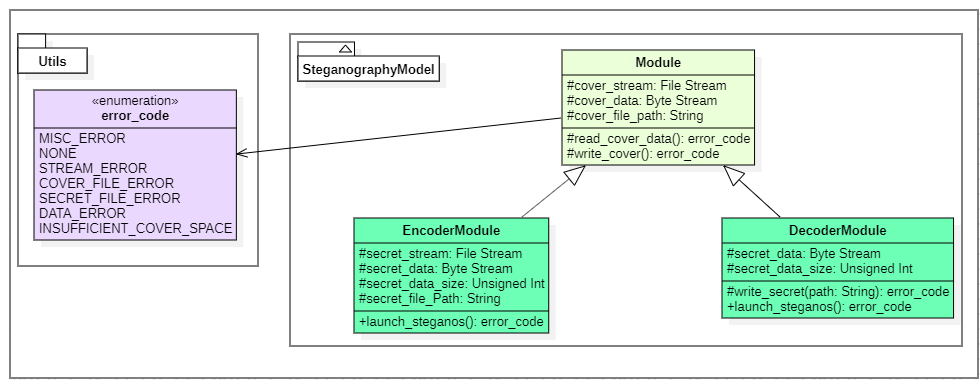
\includegraphics[width=17cm,keepaspectratio]{pics/application_chapter/diagrama_module_interface}
    \caption{Folder structure of a project using CMake}
\end{figure}

\begin{multicols*}{2}
\section{Benchmarks}

\section{Further work}
\end{multicols*}

\clearpage
\begin{multicols*}{2}
\chapter{Conclusion}
In conclusion, I believe that steganography in modern multimedia is in a really interesting position: it is not advanced enough to win over cryptography and become the main pillar behind secure communications over unreliable networks and most likely this will never change since steganography by definition will always be slower because it relies on a carrier for securing the message instead of just securing the message itself. However is steganography still an extremely important method of protecting information such that only the entrusted parties that are aware of the used algorithms will be able to extract the hidden message. It is my belief that there are countless more steganographic innovations to be made in this field that researchers will discover in the future, expanding the number of applications that steganography has right now beyond digital watermarking or Capture The Flag challenges in hacking competitions. 

Taking a step back to look at the entire known history of steganography methods we can clearly see that it has evolved a lot: from the Roman Empire hiding messages on the shaved heads of their slaves, waiting for their hair to grow back and then send them away with important messages, to the modern day digital steganography that contains several impressive and complex algorithms in order to ensure high capacity and fast encoding/decoding processes. Given this evolution it is same to assume that more and more complex and well researched algorithms will appear in the future, bringing steganography closer to the spotlight of various information security topics and conferences.
\end{multicols*}

\bibliographystyle{unsrt}
  
\bibliography{chapters/references}
\addcontentsline{toc}{chapter}{Bibliography}

\end{document}